\chapter{Development of the Prototype}\label{chapter:development_prototype}
\section{Requirements}\label{section:requirements}

In order to provide the blockchain-based weather insurance, our system must fulfill several key requirements. In this section we describe each category of requirements in a dedicated subsection.

\subsection{Functional Requirements}

\begin{itemize}
    \item \textbf{Policyholder Interaction}
    \begin{itemize}
        \item The system must provide a user interface for purchasing policies and control information such as whether a payment has been triggered or the payment status. 
        \item This user interface should be kept with minimum need
    \end{itemize}

    \item \textbf{Weather Data Integration} 
    \begin{itemize}
        \item The system must be able to receive and process global weather data from reliable and trusted external sources such as Global Surface Summary of the Day (GSOD) and Global Forecast System (GFS)
        \item Both historical and forecast data must be available
    \end{itemize}
    
    \item \textbf{Smart Contract}
    \begin{itemize}
        \item The smart contract must allow users to purchase weather-based insurance policies.
        \item The smart contract must store the policy terms, including the weather conditions that will trigger the specified amount of insurance payout.
        \item The contract must automatically trigger a payout when the predefined weather conditions are met.
    \end{itemize}
    
    \item \textbf{Oracle Integration}
    \begin{itemize}
        \item The system must use Chainlink oracles to retrieve and verify weather data from GCP datasets.
        \item Chainlink oracles must ensure secure transmission of data to the smart contract.
    \end{itemize}
    
    \item \textbf{Payout Processing}
    \begin{itemize}
        \item The system must be able to automatically execute payouts without manual intervention when the correct conditions are met.
    \end{itemize}
\end{itemize}

\subsection{Non-Functional Requirements}

\begin{enumerate}
    \item \textbf{Security}
    \begin{itemize}
        \item All the bilateral interactions between the smart contract, Chainlink oracle, google cloud and the user must be secure and tamper-proof.
    \end{itemize}
    
    \item \textbf{Scalability}
    \begin{itemize}
        \item The system must scale to handle multiple policies and users.
    \end{itemize}
    
    \item \textbf{Transparency}
    \begin{itemize}
        \item All transactions and insurance claims must be recorded on the blockchain for transparency and security.
    \end{itemize}
\end{enumerate}

\subsection{Technical Requirements (not finished)}

\begin{enumerate}
    \item \textbf{Blockchain Platform}
    \begin{itemize}
        \item The smart contract must be deployed on the Ethereum blockchain
    \end{itemize}
    
    \item \textbf{Data API}
    \begin{itemize}
        \item The system must use APIs to retrieve weather data from GCP.
    \end{itemize}
    
    \item \textbf{Chainlink Oracle}
    \begin{itemize}
        \item The system must integrate with a Chainlink node to facilitate data retrieval from GCP.
    \end{itemize}
\end{enumerate}

\section{Architecture}

In this section we will propose the architecture for our blockchain-based weather insurance system. First we present a high-level overview of the system and then elaborate on the most important components in a dedicated subsection for each component.

\subsection{General overview}

In \ref{fig:generalArchitecture} we present an overview of the general architecture that implements the requirements specified in \ref{section:requirements}. The center of the architecture is the smart contract deployed on the Ethereum blockchain. It manages all policies and decisions based on user requests and incoming weather data. The end user interacts directly with the smart contract through a decentralized app (see \ref{subsection:decentralizedApp}) where they can request insurance policies and track their contract status. 

The weather data is provided by Global Surface Summary of the Day (GSOD) and Global Forecast System (GFS) respectively. These datasets can be accessed via GCP BigQuery and GCP Storage through the GCP Interface. To bridge the gap between the off-chain data from GCP and the on-chain smart contract, the system uses a Chainlink Oracle (see \ref{subsection:ChainlinkOracle}). This Chainlink Oracle retrieves the weather data from GCP through the GCP Interface which are essentially API Endpoints and passes it on to the smart contract on the Ethereum blockchain.

\begin{figure}[h]
    \centering
    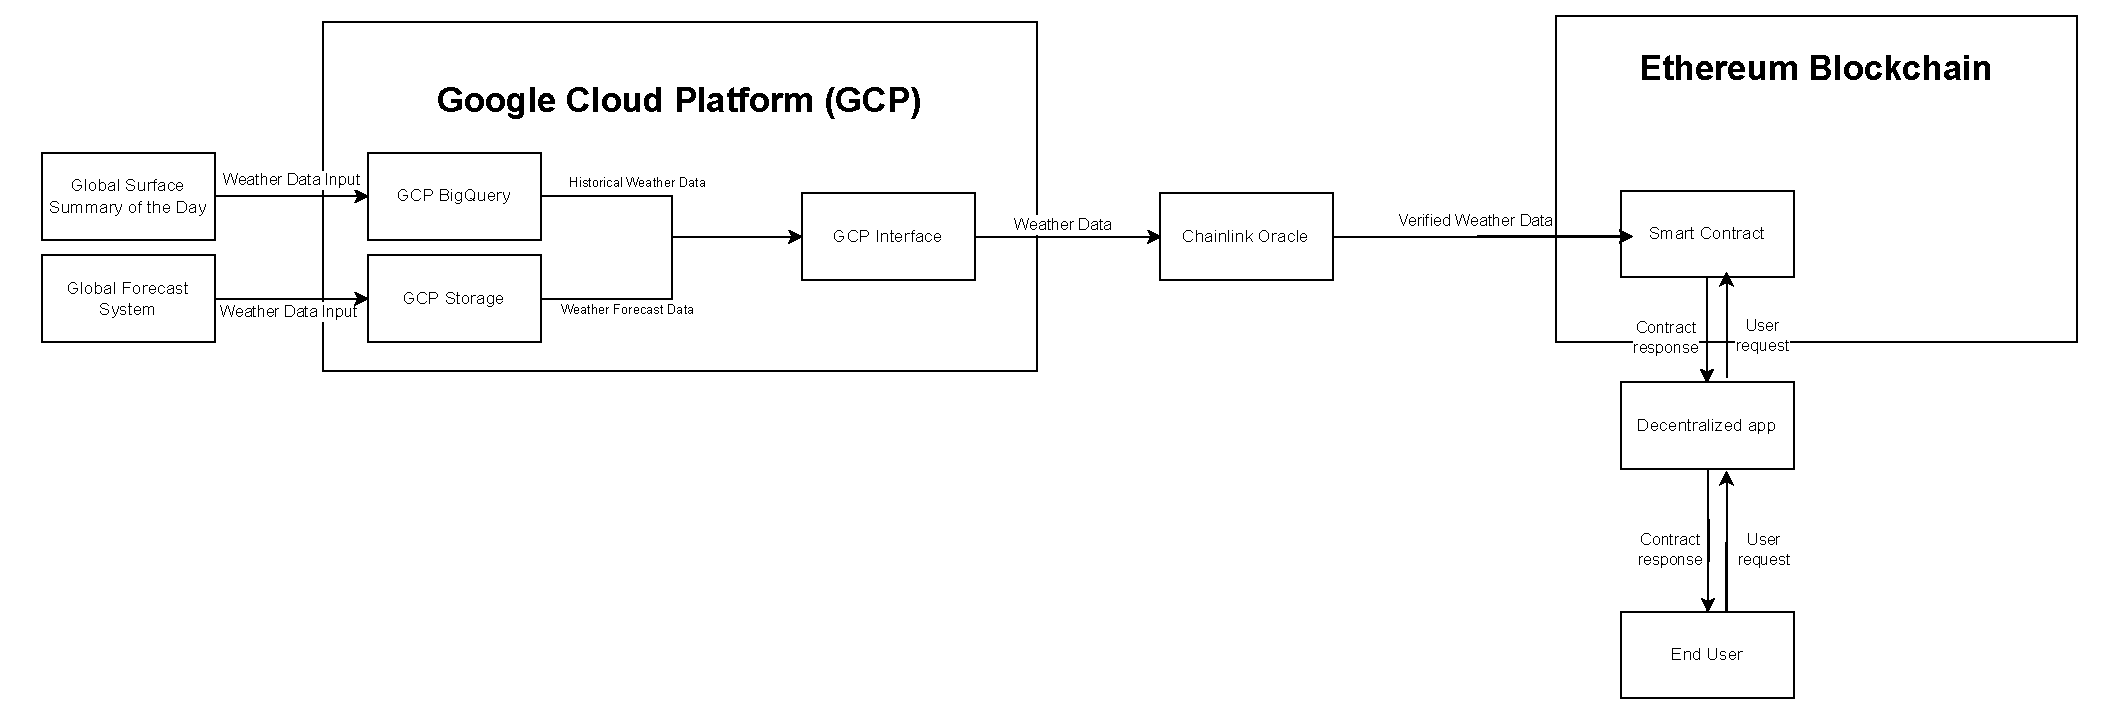
\includegraphics[width=0.8\textwidth]{figures/architecture-overview.drawio.pdf}
    \caption{Diagram showing the architecture of the smart contract. \textit{Source: Author's own representation.}}
    \label{fig:generalArchitecture}
\end{figure}

\subsection{Decentralized app}\label{subsection:decentralizedApp}

The decentralized application (DApp) allows a non-technical user to directly interact with the blockchain. Through its interface a user can request insurance policies, check policy statuses and receive notifications. Unlike traditional applications, which interact with a centrally managed backend, decentralized applications interact directly with a smart contract on a blockchain.

This interaction requires a digital wallet (e.g. MetaMask) which enables the user to initiate and sign a transaction when making a request, such as purchasing an insurance policy. In our architecture, the dApp serves as the primary interface in order for the end-users to interact with the system. 

(Idea: Include a mockup of a frontend utilizing metamask)

\subsection{Integration of chainlink oracles and GCP}\label{subsection:ChainlinkOracle}

Since the weater data from GSOD and GFS, which is accessed through the Google Cloud Platform (GCP), is not directly available from the on-chain environment of the smart contract we need to leverage oracles, which retreive and verify external data before delivering it to the blockchain.

In this case, Chainlink oracles are used to securely interact with the Google Cloud Platform (GCP) and pass it to the smart contract. The Chainlink oracle network consists of globally distributed nodes. When a request is triggered, multiple nodes independently access GCP and receive the weather data specified in the request. If any nodes return results that differ from the majority, they are flagged as potentially malicious. This decentralized approach ensures that only verified and reliable weather data is passed on to the smart contract.


\section{Data flow}

In this section, we examine the two primary data flow scenarios central to our blockchain-based weather insurance system: the process of purchasing a weather insurance policy (see \cref{subsection:purchasePolicyFlow}) and the process of triggering a policy payout (see \cref{subsection:policyPayoutTrigger}). These scenarios represent the fundamental interactions between the end user, the smart contract and the external data sources. In the subsequent chapters we elaborate on the core functionalities utilized in the two scenarios such as the process of retreiving weather data and the calculating of the policy conditions.

\subsection{Purchase weather insurance policy}\label{subsection:purchasePolicyFlow}

The flow diagram in \cref{fig:purchasePolicyFlow} outlines the steps involved in purchasing a weather insurance policy in out system. The main components involved are the End User, Smart Contract, Chainlink Oracle and the Google Cloud Platform (GCP). Each of these components play a central role in enabling the policy purchase and the associated data retrieval and validation processes. Every request between components includes a set of parameters. These parameters contain the necessary information that each component needs in order to perform its role and functions accurately. For example, in a purchase policy request parameters such as location, coverage duration and type of coverage are sent to the smart contract. Table \cref{tab:flowRequests} contains all requests with their respective parameters.

\begin{figure}[h]
    \centering
    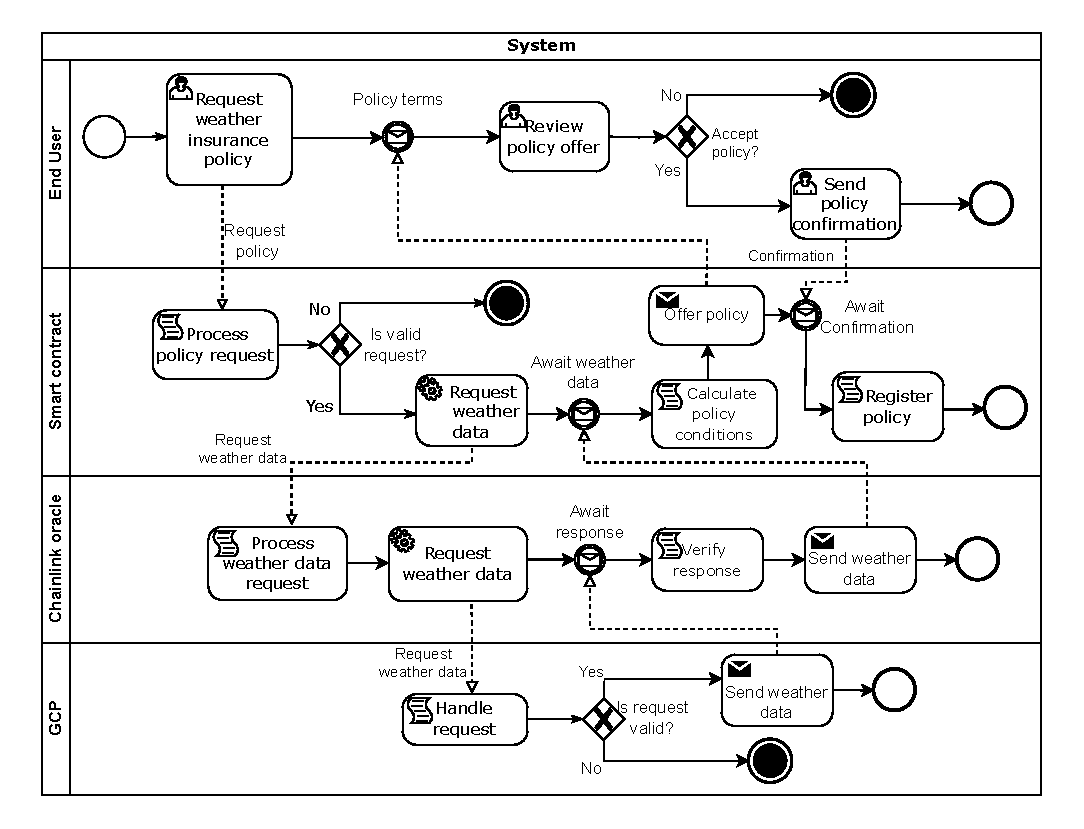
\includegraphics[width=0.95\textwidth]{figures/flow-purchase-policy.drawio.pdf}
    \caption{Purchase policy flow \textit{Source: Author's own representation.}}
    \label{fig:purchasePolicyFlow}
\end{figure}

\begin{table}[h]
    \centering
    \renewcommand{\arraystretch}{1.3}
\begin{tabular}{|>{\centering\arraybackslash}m{2cm}|>{\centering\arraybackslash}p{5cm}|>{\centering\arraybackslash}m{5cm}|>{\centering\arraybackslash}m{3cm}|}
    \hline
    \textbf{Name} & \textbf{Parameters} & \textbf{Description} & \textbf{Response} \\ 
    \hline
    Request policy & \makecell{Location: String \\ Coverage start date: Date \\ Coverage end date: Date \\ Type of coverage: Enum}  & Requests a policy with the given parameters as the underlying conditions & Binding policy offer including financial conditions and a unique policy ID\\ 
    \hline
    Request weather data & \makecell{Location: String \\ Weather start date: Date \\ Weather end date: Date \\ Type of weather data: Enum \\ Frequency: Enum \\ Data Type: Enum} & Requests weather data in a specific date range. Examples for weather data types are rainfall, wind speed and temperature. Frequency indicates the data granularity (e.g. hourly, daily). Data Type can be either forecast or historical. &  Weather data in JSON format \\ 
    \hline
    Confirmation & \makecell{Policy ID: String \\ Confirmed: Boolean} & Sends a confirmation to the smart contract with the specific policy ID & - \\ 
    \hline
\end{tabular}
    \caption{Requests with their parameters \textit{Source: Author's own representation.}}
    \label{tab:flowRequests}
\end{table}

The End User starts the process by requesting a weather insurance policy from the smart contract. This interaction happens through the use of a decentralized app (dApp) \cref{subsection:decentralizedApp}, which is not explicitly mentioned in the diagram but can be thought of as the interface enabling the end user to interact directly with the smart contract. Through the dApp the user requests a weather insurance policy. In table \cref{tab:flowRequests} we find the detailed description of each request. In the policy request the user has to specify the conditions of the policy, these include the location, start- and end-date as well the type of coverage (for example drought coverage or storm coverage).

The smart contract then fetches the necessary weather data needed for the calculation of the policy conditions by sending a request to the Chainlink oracle containing the necessary parameters (see "Weather data request" in table \cref{tab:flowRequests}). The Chainlink oracle then propagates this request to the Google Cloud Platform. Due to the decentralized nature of Chainlink oracles this request is sent multiple times to the GCP from different Chainlink nodes (see \cref{subsection:ChainlinkOracle}). The responses from each of these requests are then analyzed and verified by the Chainlink network and sent back to the Smart Contract. The Smart Contract then calculates the policy conditions (such as the premium and the payout sum tied to the weather conditions) and sends an offer to the end user. If the end user accepts the terms offered by the Smart Contract, then the policy is valid and registered on the blockchain.

Note that in the diagram there are two "Request weather data" requests depicted. One is from the Smart Contract to the Chainlink oracle and one from the Chainlink oracle to the GCP. Even though the requests differ in their technical details (such as type of request and authorization headers) we have combined them in table \cref{tab:flowRequests} as one entry. This was chosen specifically for simplicity purposes, since the diagram is an abstraction of a policy purchase process and leaves space for flexibility in technical implementation.

\subsection{Policy payout trigger}\label{subsection:policyPayoutTrigger}

The second main flow is shown in \cref{fig:payoutFlow}. It presents the process of triggering a policy payout. This payout happens when the specified policy conditions from \cref{subsection:purchasePolicyFlow} are fulfilled (assuming a policy has been agreed upon between the end user and the smart contract). 

A key decision in the design of the payout process is determining is what triggers an eligibility check and the following payout process. A possible solution would be to use scheduled tasks that periodically trigger an eligibility request on every policy held by the Smart Contract. Since the Ethereum Blockchain does not support scheduled or automated tasks natively such a solution would require an external solution. For example Chainlink offers an automation service \autocite{chainlink_automation} with which it would be possible to trigger a scheduled eligibility check on the Smart Contract (e.g. once a day). This service would however cost gas which has to be paid by the Smart Contract and result in a lot of unnecessary transactions. In our proposed solution, the end user initiates the eligibility check instead. This decision prioritizes simplicity and cost-efficiency, avoiding extra transactions that would otherwise increase the policy premium for the end user.

After the end user has initiated the eligibility check through the use of a decentralized App (dApp), the Smart Contract gathers the weather data for the specific location and covered duration of the policy. This process of retrieving the relevant weather data is similar to the one in \cref{subsection:purchasePolicyFlow}, with the key distinciton being that the weather data contains past data and not forecast data. Once the weather data is received, the smart contract evaluates whether the conditions for a payout are met and communicates the outcome to the end user. If the end user is eligible for a payout, they can submit a request to the smart contract, which will then transfer the agreed-upon funds as specified in the policy.


\begin{figure}[h]
    \centering
    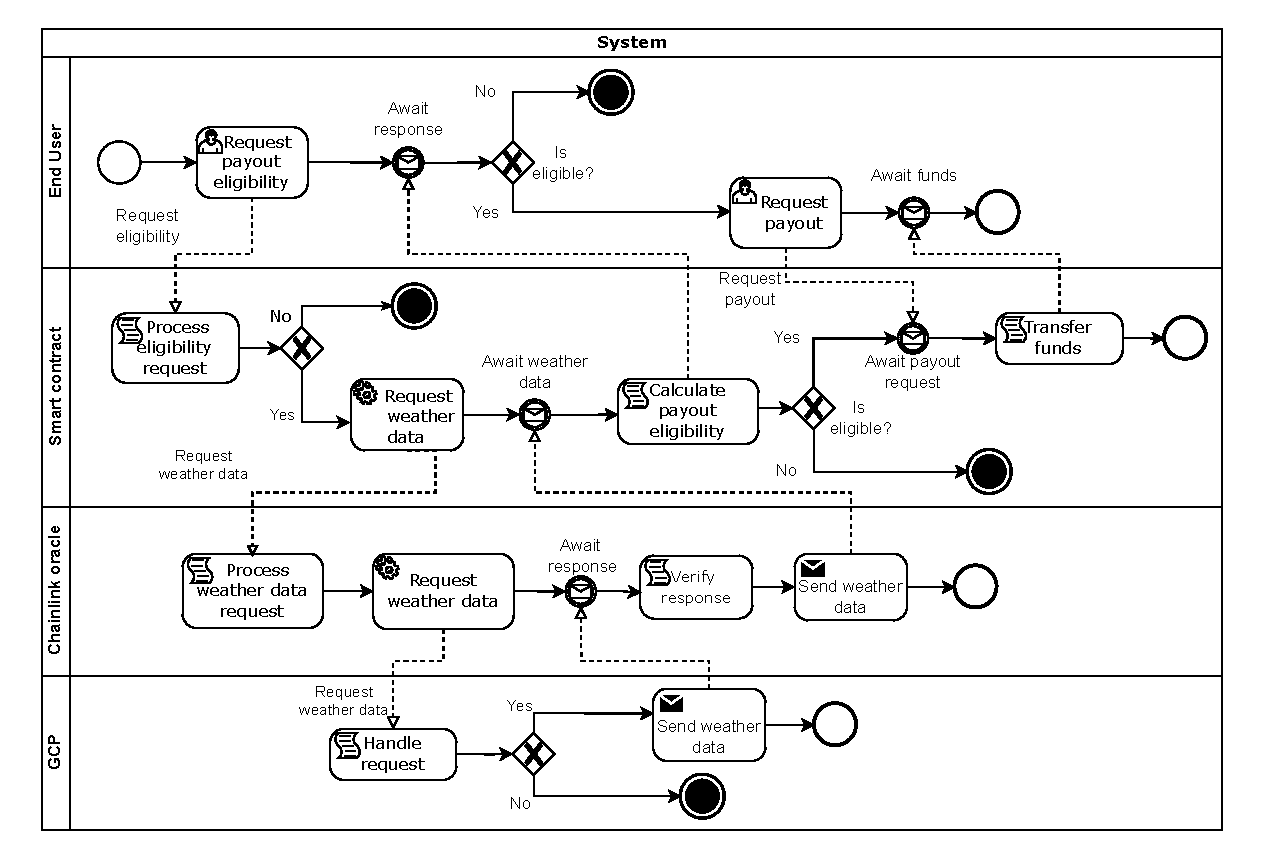
\includegraphics[width=0.95\textwidth]{figures/flow-policy-payout-trigger.drawio.pdf}
    \caption{Payout flow \textit{Source: Author's own representation.}}
    \label{fig:payoutFlow}
\end{figure}

\begin{table}[h]
    \centering
    \renewcommand{\arraystretch}{1.3}
\begin{tabular}{|>{\centering\arraybackslash}m{2cm}|>{\centering\arraybackslash}p{5cm}|>{\centering\arraybackslash}m{5cm}|>{\centering\arraybackslash}m{3cm}|}
    \hline
    \textbf{Name} & \textbf{Parameters} & \textbf{Description} & \textbf{Response} \\ 
    \hline
    Request eligibility & \makecell{Policy ID: String}  & Requests an eligibility check, which is then performed by the smart contract. & Whether the policy is eligible for a payout or not in JSON format. \\
    \hline
    Request weather data & \makecell{Location: String \\ Weather start date: Date \\ Weather end date: Date \\ Type of weather data: Enum \\ Frequency: Enum \\ Data Type: Enum} & Requests weather data in a specific date range. Examples of weather data types include rainfall, wind speed, and temperature. Frequency indicates the data granularity (e.g. hourly, daily). Data Type can be either forecast or historical. &  Weather data in JSON format. \\ 
    \hline
    Request payout & \makecell{Policy ID: String} & Requests the payout of funds. & Amount of funds specified in the policy. \\ 
    \hline
\end{tabular}
    \caption{Requests with their parameters \textit{Source: Author's own representation.}}
    \label{tab:payoutFlowRequests}
\end{table}

\subsection{Interaction with smart contract}

As mentioned in \cref{subsection:purchasePolicyFlow} and \cref{subsection:policyPayoutTrigger}, the end user communicates with the Smart Contract through a decentralized App (see \cref{subsection:decentralizedApp}). The dApp interface is indistinguishable from a regular app interface, with the key difference being that it interacts directly with the blockchain. Within the dApp the end user can create the requests and enter the relevant parameters. Once the user submits a request, the dApp creates a transaction that is signed using the end user's digital wallet. This transaction is then broadcasted to the blockchain, where it can interact directly with the smart contract.

\subsection{Calculating policy conditions}

One of the core functions of tghe smart contract is calculating the policy conditions.


\subsection{Smart contract fetching weather data}